% Thermoelectric figure of merit $zT$ vs carrier concentration $n$ for \ch{Bi2Te3} based on empirical data in ref.~\cite{rowe_alpha-sigma_1995}. Tuning $n$ for optimal $zT$ involves a compromise between thermal conductivity $\kappa$, Seebeck coefficient $S$ and electrical conductivity $\sigma$. Increasing the electrical conductivity $\sigma$ not only produces an increase in the electronic thermal conductivity $\kappa_\text{el}$ but also usually decreases the Seebeck coefficient $S$. This makes optimal $\zT$ difficult to achieve. Plot scales are $\kappa/\si{\watt\per\meter\per\kelvin} \in [0,10]$, $S/\si{\micro\volt\per\kelvin} \in [0,500]$, $\sigma/\si{\per\ohm\per\centi\meter} \in [0,5000]$.

\documentclass[tikz]{standalone}

\usepackage{pgfplots,siunitx}

\pgfplotsset{compat=newest}

\begin{document}
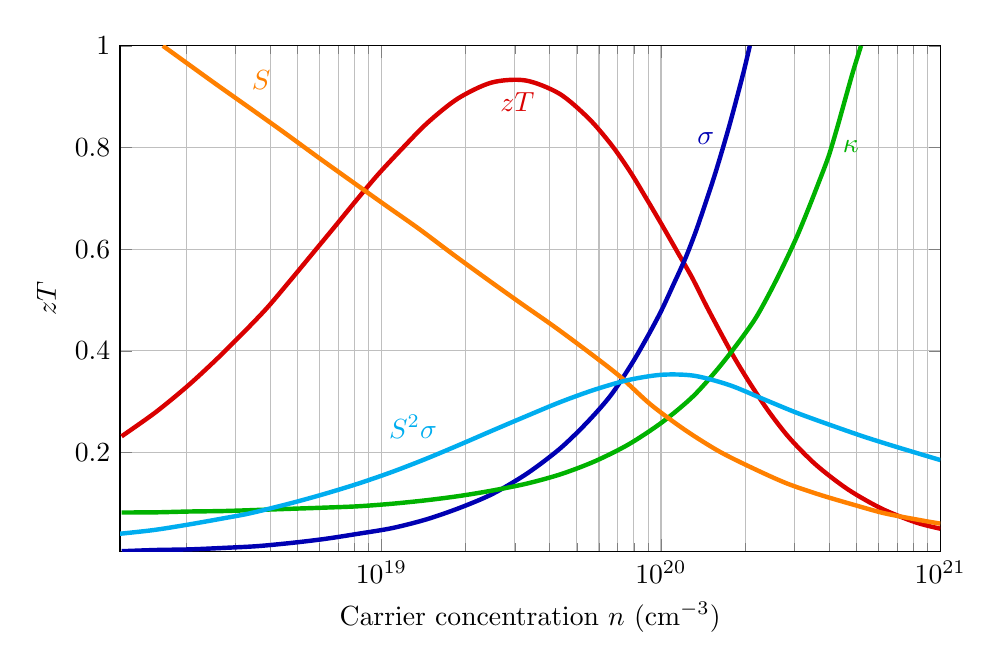
\begin{tikzpicture}
  \begin{axis}[
      xmode=log,
      domain=1e17:1e21,
      ymax=1,
      enlargelimits=false,
      ylabel=$zT$,
      xlabel=Carrier concentration $n$ (\si{\per\centi\meter\cubed}),
      grid=both,
      width=12cm,
      height=8cm,
      decoration={name=none},
    ]
    \addplot [ultra thick, smooth, red!85!black] coordinates {
        (1.174e+18, 0.2317)
        (1.551e+18, 0.2787)
        (2.016e+18, 0.3300)
        (2.549e+18, 0.3816)
        (3.171e+18, 0.4332)
        (3.891e+18, 0.4842)
        (4.697e+18, 0.5373)
        (5.623e+18, 0.5892)
        (6.714e+18, 0.6404)
        (8.017e+18, 0.6923)
        (9.650e+18, 0.7450)
        (1.178e+19, 0.7963)
        (1.461e+19, 0.8486)
        (1.878e+19, 0.8964)
        (2.481e+19, 0.9278)
        (3.279e+19, 0.9318)
        (4.334e+19, 0.9057)
        (5.515e+19, 0.8571)
        (6.662e+19, 0.8045)
        (7.767e+19, 0.7519)
        (8.859e+19, 0.7000)
        (1.008e+20, 0.6476)
        (1.143e+20, 0.5953)
        (1.290e+20, 0.5449)
        (1.447e+20, 0.4906)
        (1.628e+20, 0.4374)
        (1.837e+20, 0.3850)
        (2.101e+20, 0.3327)
        (2.436e+20, 0.2799)
        (2.887e+20, 0.2281)
        (3.594e+20, 0.1753)
        (4.674e+20, 0.1271)
        (6.178e+20, 0.08917)
        (8.167e+20, 0.06240)
        (1e+21, 0.05)
      } node[pos=0.48, anchor=north] {$zT$};
    \addplot [ultra thick, smooth, blue!70!black] coordinates {
        (1.176e+18, 0.005689)
        (1.554e+18, 0.008070)
        (2.054e+18, 0.009285)
        (2.714e+18, 0.01216)
        (3.587e+18, 0.01561)
        (4.740e+18, 0.02190)
        (6.264e+18, 0.02984)
        (8.277e+18, 0.04013)
        (1.094e+19, 0.05127)
        (1.445e+19, 0.06820)
        (1.910e+19, 0.09120)
        (2.511e+19, 0.1191)
        (3.333e+19, 0.1593)
        (4.344e+19, 0.2072)
        (5.433e+19, 0.2587)
        (6.613e+19, 0.3123)
        (7.852e+19, 0.3739)
        (8.925e+19, 0.4266)
        (1.001e+20, 0.4779)
        (1.110e+20, 0.5310)
        (1.224e+20, 0.5824)
        (1.335e+20, 0.6359)
        (1.441e+20, 0.6893)
        (1.551e+20, 0.7425)
        (1.660e+20, 0.7960)
        (1.767e+20, 0.8478)
        (1.876e+20, 0.9009)
        (1.986e+20, 0.9532)
        (2.08e+20, 1)
      } node[pos=0.95, anchor=east] {$\sigma$};
    \addplot [ultra thick, smooth, green!70!black] coordinates {
        (1.175e+18, 0.08187)
        (1.553e+18, 0.08218)
        (2.053e+18, 0.08379)
        (2.713e+18, 0.08472)
        (3.585e+18, 0.08684)
        (4.738e+18, 0.08916)
        (6.261e+18, 0.09142)
        (8.274e+18, 0.09411)
        (1.093e+19, 0.09912)
        (1.445e+19, 0.1059)
        (1.909e+19, 0.1145)
        (2.523e+19, 0.1256)
        (3.334e+19, 0.1391)
        (4.405e+19, 0.1576)
        (5.821e+19, 0.1830)
        (7.691e+19, 0.2164)
        (1.016e+20, 0.2605)
        (1.302e+20, 0.3102)
        (1.589e+20, 0.3629)
        (1.882e+20, 0.4143)
        (2.181e+20, 0.4641)
        (2.472e+20, 0.5181)
        (2.764e+20, 0.5714)
        (3.066e+20, 0.6246)
        (3.363e+20, 0.6780)
        (3.669e+20, 0.7310)
        (3.981e+20, 0.7826)
        (4.273e+20, 0.8389)
        (4.560e+20, 0.8942)
        (4.868e+20, 0.9493)
        (5.2e+20, 1)
      } node[pos=0.95, anchor=west] {$\kappa$};
    \addplot [ultra thick, smooth, orange] coordinates {
        (1.65e+18, 1)
        (1.931e+18, 0.9729)
        (2.553e+18, 0.9248)
        (3.375e+18, 0.8777)
        (4.462e+18, 0.8302)
        (5.899e+18, 0.7816)
        (7.745e+18, 0.7351)
        (1.031e+19, 0.6866)
        (1.363e+19, 0.6397)
        (1.802e+19, 0.5897)
        (2.382e+19, 0.5412)
        (3.149e+19, 0.4937)
        (4.162e+19, 0.4471)
        (5.503e+19, 0.3977)
        (7.117e+19, 0.3500)
        (9.181e+19, 0.2944)
        (1.224e+20, 0.2436)
        (1.618e+20, 0.2019)
        (2.138e+20, 0.1687)
        (2.826e+20, 0.1389)
        (3.736e+20, 0.1161)
        (4.938e+20, 0.09646)
        (6.321e+20, 0.08022)
        (8.578e+20, 0.06624)
        (1e+21, 0.06)
      } node[pos=0.1, anchor=south west] {$S$};
    \addplot [ultra thick, smooth, cyan] coordinates {
        (1.159e+18, 0.04006)
        (1.532e+18, 0.04739)
        (2.025e+18, 0.05790)
        (2.676e+18, 0.06974)
        (3.386e+18, 0.08033)
        (4.675e+18, 0.09928)
        (6.179e+18, 0.1176)
        (8.168e+18, 0.1379)
        (1.080e+19, 0.1608)
        (1.427e+19, 0.1864)
        (1.886e+19, 0.2142)
        (2.492e+19, 0.2430)
        (3.294e+19, 0.2713)
        (4.353e+19, 0.2989)
        (5.754e+19, 0.3230)
        (7.605e+19, 0.3422)
        (1.005e+20, 0.3528)
        (1.314e+20, 0.3509)
        (1.757e+20, 0.3326)
        (2.327e+20, 0.3049)
        (3.071e+20, 0.2777)
        (4.061e+20, 0.2535)
        (5.369e+20, 0.2304)
        (7.098e+20, 0.2095)
        (1e+21, 0.185)
      } node[pos=0.4, anchor=south east] {$S^2 \sigma$};
  \end{axis}
\end{tikzpicture}
\end{document}